In this section we document the results corresponding to \intlumi data, for 
cut-based analysis and the shape based analyses based on both 
$M_T$ variable and the matrix element outputs. 

Tables~\ref{tab:yield_cutbased}-\ref{tab:yield_me_shapebased} shows the signal and background expectations 
in ee and $\mu\mu$ final states for the cut-based analysis and shape analysis based on $M_T$ variable 
and matrix element output. The Higgs boson mass dependent signal selections are described in Section~\ref{sec:signal_selection}.
The observed and expected cross section ratio limits as a function of the Higgs mass, together with the 1/2-$\sigma$ uncertainty bands 
are shown in Table~\ref{tab:limits_5fb} and Figure~\ref{fig:limits_5fb} for these three analyses. 
The corresponding $M_T$ and matrix element output distributions are shown in Appendix~\ref{app:mtshape} and Appendix~\ref{app:meshape} respectively.

With the current data sample, we expect to exclude the standard model Higgs boson 
in the mass range of about [300,450]~\GeVcc in the cut-based analysis, compared with the 
expected exclusion range of [300,475]~\GeVcc. 
The observed exclusion region extends to about [275-455]~\GeVcc using shape analysis based on 
$M_T$ variable, compared to the expected exclusion range of [290-490]~\GeVcc.
The observed exclusion region extends to about [300-500]~\GeVcc using shape analysis based on 
matrix element output, compared to the expected exclusion range of [280-480]~\GeVcc.


%%%%%%%%%%%%%%%%%%%%%%%%%
\begin{table}[!htbp]
{\scriptsize
\begin{center}
 \begin{tabular}{l | c c |  c c c c c c | c }
 \hline\hline
 $m_H$ & qqH & ggH & qqZZ & ggZZ & WZ & WWTop & Zjets & $\sum$Bkg & Data \\
 \hline
\multicolumn{10}{c} {ee} \\ \hline
250 & $0.9\pm0.1$ & $8.2\pm1.2$ & $13.2\pm1.4$ & $1.2\pm0.3$ & $9.7\pm1.2$ & $29.4\pm3.6$ & $6.0\pm6.0$ & $59.5\pm6.3$ & 58 \\
300 & $0.9\pm0.1$ & $7.9\pm1.2$ & $8.7\pm0.9$ & $0.8\pm0.2$ & $5.3\pm0.7$ & $9.6\pm2.1$ & $3.0\pm3.0$ & $27.3\pm3.2$ & 20 \\
350 & $0.7\pm0.1$ & $8.0\pm1.3$ & $6.2\pm0.7$ & $0.5\pm0.1$ & $2.8\pm0.4$ & $0.9\pm0.7$ & $1.7\pm1.7$ & $12.2\pm1.9$ & 10 \\
400 & $0.5\pm0.1$ & $6.7\pm1.2$ & $4.6\pm0.5$ & $0.4\pm0.1$ & $1.9\pm0.3$ & $0.0\pm0.4$ & $1.0\pm1.0$ & $8.0\pm1.2$ & 7 \\
500 & $0.3\pm0.1$ & $2.9\pm0.7$ & $2.8\pm0.3$ & $0.2\pm0.0$ & $0.9\pm0.1$ & $0.0\pm0.4$ & $0.5\pm0.5$ & $4.4\pm0.6$ & 5 \\
600 & $0.2\pm0.1$ & $1.1\pm0.4$ & $1.4\pm0.2$ & $0.1\pm0.0$ & $0.4\pm0.1$ & $0.0\pm0.4$ & $0.3\pm0.3$ & $2.2\pm0.3$ & 0 \\
\hline
\multicolumn{10}{c} {$\mu\mu$} \\ 
\hline
250 & $1.3\pm0.1$ & $11.7\pm1.7$ & $19.6\pm1.9$ & $1.8\pm0.4$ & $14.4\pm1.7$ & $36.5\pm4.5$ & $8.6\pm8.6$ & $81.0\pm9.0$ & 82 \\
300 & $1.2\pm0.1$ & $11.2\pm1.6$ & $12.7\pm1.2$ & $1.1\pm0.2$ & $7.5\pm0.9$ & $11.7\pm2.5$ & $4.4\pm4.4$ & $37.4\pm4.6$ & 41 \\
350 & $1.0\pm0.1$ & $11.0\pm1.7$ & $8.5\pm0.8$ & $0.7\pm0.2$ & $4.3\pm0.5$ & $1.1\pm0.7$ & $2.6\pm2.6$ & $17.2\pm2.8$ & 17 \\
400 & $0.7\pm0.1$ & $9.4\pm1.6$ & $6.6\pm0.7$ & $0.5\pm0.1$ & $2.8\pm0.3$ & $0.0\pm0.4$ & $1.6\pm1.6$ & $11.6\pm1.8$ & 11 \\
500 & $0.4\pm0.1$ & $3.9\pm0.9$ & $4.2\pm0.4$ & $0.3\pm0.1$ & $1.2\pm0.2$ & $0.0\pm0.4$ & $0.8\pm0.8$ & $6.5\pm0.9$ & 9 \\
600 & $0.2\pm0.1$ & $1.5\pm0.5$ & $2.2\pm0.2$ & $0.2\pm0.0$ & $0.5\pm0.1$ & $0.0\pm0.4$ & $0.3\pm0.3$ & $3.2\pm0.4$ & 5 \\
\hline\hline
\end{tabular}
\end{center}
}
\caption{Number of events observed in data and the expected signal and background yields 
	for an integrated luminosity of \intlumi 
	after applying the higgs selections in the {\bf cut-based analysis}.}	
%	For the sum of the $\ww$ and Top backgrounds, the uncertainties are modelled by a Gamma function of the number 
%	of $e\mu$ events in the control region.  }
\label{tab:yield_cutbased}
\end{table}
%%%%%%%%%%%%%%%%%%%%%%%%%%%%%%%

%%%%%%%%%%%%%%%%%%%%%%%%%
\begin{table}[!htbp]
{\scriptsize
 \begin{center}
 \begin{tabular}{l | c c | c c c c c c  | c}
 \hline\hline
 $mH$ & qqH & ggH & ZZ & ggZZ & WZ & WW/Top & Zjets & $\sum$Bkg & Data \\
 \hline
\multicolumn{10}{c} {ee} \\ 
\hline
250 & $1.0\pm0.1$ & $8.7\pm1.3$ & $18.0\pm1.9$ & $1.7\pm0.4$ & $14.4\pm1.8$ & $49.3\pm4.7$ & $14.5\pm14.5$ & $97.9\pm15.5$ & 95 \\
300 & $1.0\pm0.1$ & $9.1\pm1.4$ & $12.9\pm1.4$ & $1.1\pm0.3$ & $7.8\pm1.0$ & $17.0\pm2.8$ & $4.4\pm4.4$ & $43.2\pm5.5$ & 32 \\
350 & $1.0\pm0.1$ & $10.4\pm1.7$ & $14.9\pm1.6$ & $1.3\pm0.3$ & $8.7\pm1.1$ & $17.0\pm2.8$ & $5.0\pm5.0$ & $46.8\pm6.0$ & 35 \\
400 & $0.7\pm0.1$ & $8.8\pm1.5$ & $15.9\pm1.7$ & $1.4\pm0.3$ & $9.1\pm1.2$ & $17.0\pm2.8$ & $5.2\pm5.2$ & $48.5\pm6.2$ & 39 \\
500 & $0.4\pm0.1$ & $4.0\pm1.0$ & $17.0\pm1.8$ & $1.5\pm0.3$ & $9.4\pm1.2$ & $17.0\pm2.8$ & $5.4\pm5.4$ & $50.3\pm6.5$ & 39 \\
600 & $0.3\pm0.1$ & $1.7\pm0.6$ & $17.3\pm1.8$ & $1.5\pm0.3$ & $9.5\pm1.2$ & $17.0\pm2.8$ & $5.4\pm5.4$ & $50.8\pm6.5$ & 39 \\
\hline
\multicolumn{10}{c} {$\mu\mu$} \\ 
\hline
250 & $1.5\pm0.1$ & $12.4\pm1.8$ & $26.9\pm2.6$ & $2.5\pm0.5$ & $21.4\pm2.5$ & $61.5\pm5.8$ & $21.7\pm21.7$ & $133.9\pm22.8$ & 140 \\
300 & $1.4\pm0.1$ & $12.9\pm1.9$ & $18.8\pm1.8$ & $1.7\pm0.4$ & $11.2\pm1.3$ & $21.2\pm3.4$ & $7.0\pm7.0$ & $59.9\pm8.2$ & 60 \\
350 & $1.3\pm0.1$ & $14.8\pm2.3$ & $21.5\pm2.1$ & $1.9\pm0.4$ & $12.5\pm1.5$ & $21.2\pm3.4$ & $7.9\pm7.9$ & $65.0\pm9.0$ & 62 \\
400 & $1.0\pm0.1$ & $12.6\pm2.2$ & $23.1\pm2.3$ & $2.0\pm0.4$ & $13.1\pm1.5$ & $21.2\pm3.4$ & $8.2\pm8.2$ & $67.6\pm9.3$ & 65 \\
500 & $0.6\pm0.1$ & $5.5\pm1.3$ & $24.9\pm2.4$ & $2.2\pm0.5$ & $13.5\pm1.6$ & $21.2\pm3.4$ & $8.5\pm8.5$ & $70.2\pm9.6$ & 70 \\
600 & $0.3\pm0.1$ & $2.3\pm0.8$ & $25.3\pm2.5$ & $2.2\pm0.5$ & $13.6\pm1.6$ & $21.2\pm3.4$ & $8.6\pm8.6$ & $70.8\pm9.7$ & 70 \\
\hline\hline
\end{tabular}
\end{center}
}
\caption{Number of events observed in data and the expected signal and background yields for 
	an integrated luminosity of \intlumi after applying the higgs selections in the 
	{\bf shape analysis based on $M_T$}. }
\label{tab:yield_mt_shapebased}
\end{table}
%%%%%%%%%%%%%%%%%%%%%%%%%%%%%%%

%%%%%%%%%%%%%%%%%%%%%%%%%
\begin{table}[!htbp]
{\scriptsize
 \begin{center}
 \begin{tabular}{l | c c | c c c c c c | c}
 \hline\hline
 $mH$ & qqH & ggH & ZZ & ggZZ & WZ & WW/Top & Zjets & $\sum$Bkg & Data \\
 \hline
\multicolumn{10}{c} {ee} \\ 
\hline
250 & $1.1\pm0.1$ & $8.9\pm1.3$ & $27.4\pm2.9$ & $2.4\pm0.5$ & $18.7\pm2.3$ & $54.7\pm4.9$ & $18.9\pm18.9$ & $122.1\pm19.9$ & 115 \\
300 & $1.2\pm0.1$ & $10.3\pm1.6$ & $22.4\pm2.4$ & $2.0\pm0.4$ & $14.3\pm1.8$ & $38.9\pm4.2$ & $11.5\pm11.5$ & $89.1\pm12.6$ & 84 \\
350 & $1.0\pm0.1$ & $10.8\pm1.7$ & $18.2\pm1.9$ & $1.6\pm0.4$ & $10.6\pm1.3$ & $22.6\pm3.2$ & $8.1\pm8.1$ & $61.2\pm9.0$ & 58 \\
400 & $0.7\pm0.1$ & $9.3\pm1.6$ & $18.2\pm1.9$ & $1.6\pm0.4$ & $10.6\pm1.3$ & $22.6\pm3.2$ & $8.1\pm8.1$ & $61.2\pm9.0$ & 58 \\
500 & $0.4\pm0.1$ & $4.2\pm1.0$ & $14.8\pm1.6$ & $1.3\pm0.3$ & $8.0\pm1.0$ & $14.3\pm2.5$ & $5.9\pm5.9$ & $44.3\pm6.7$ & 47 \\
600 & $0.2\pm0.1$ & $1.6\pm0.6$ & $9.9\pm1.0$ & $0.8\pm0.2$ & $4.6\pm0.6$ & $3.6\pm1.3$ & $3.4\pm3.4$ & $22.4\pm3.9$ & 26 \\
\hline
\multicolumn{10}{c} {$\mu\mu$} \\ 
\hline
250 & $1.5\pm0.1$ & $12.8\pm1.8$ & $40.3\pm3.9$ & $3.6\pm0.8$ & $27.6\pm3.2$ & $68.1\pm6.1$ & $27.9\pm27.9$ & $167.5\pm29.1$ & 173 \\
300 & $1.7\pm0.1$ & $14.8\pm2.2$ & $33.2\pm3.2$ & $2.9\pm0.6$ & $20.8\pm2.4$ & $48.1\pm5.2$ & $17.1\pm17.1$ & $122.1\pm18.3$ & 125 \\
350 & $1.4\pm0.1$ & $15.3\pm2.4$ & $26.8\pm2.6$ & $2.3\pm0.5$ & $15.6\pm1.8$ & $28.2\pm3.9$ & $12.0\pm12.0$ & $85.0\pm13.1$ & 89 \\
400 & $1.0\pm0.1$ & $13.3\pm2.3$ & $26.8\pm2.6$ & $2.3\pm0.5$ & $15.6\pm1.8$ & $28.2\pm3.9$ & $12.0\pm12.0$ & $85.0\pm13.1$ & 89 \\
500 & $0.6\pm0.1$ & $5.6\pm1.3$ & $21.6\pm2.1$ & $1.8\pm0.4$ & $11.8\pm1.4$ & $17.8\pm3.2$ & $8.8\pm8.8$ & $61.8\pm9.7$ & 63 \\
600 & $0.3\pm0.1$ & $2.3\pm0.8$ & $14.2\pm1.4$ & $1.2\pm0.3$ & $6.7\pm0.8$ & $4.5\pm1.6$ & $5.0\pm5.0$ & $31.7\pm5.5$ & 34 \\
\hline\hline
\end{tabular}
\end{center}
}
\caption{Number of events observed in data and the expected signal and background yields for an integrated 
	luminosity of \intlumi 	after applying the higgs selections in the 
	{\bf shape analysis based on matrix element output$M_T$}. }
\label{tab:yield_me_shapebased}
\end{table}
%%%%%%%%%%%%%%%%%%%%%%%

%%%%%%%%%%%%%%%%%%%%%%%%%%%%%%%
\begin{table}[!htbp]
\begin{center}
\begin{tabular}{ccccc}
\hline\hline
Mass & Observed & Median Expected & [-$\sigma$, +$\sigma$] & [-2$\sigma$, +2$\sigma$]\\\hline
\hline
\multicolumn{5}{c} {Cut-based Analysis} \\ 
\hline
250 & 1.62 & 1.62 & [1.17, 2.24] & [0.88, 2.98] \\
300 & 0.95 & 1.04 & [0.75, 1.44] & [0.56, 1.91] \\
350 & 0.60 & 0.68 & [0.49, 0.94] & [0.37, 1.25] \\
400 & 0.59 & 0.65 & [0.47, 0.91] & [0.35, 1.21] \\
500 & 1.61 & 1.19 & [0.86, 1.66] & [0.65, 2.20] \\
600 & 2.20 & 2.36 & [1.70, 3.28] & [1.28, 4.36] \\
\hline
\multicolumn{5}{c} {Shape Analysis Based on $M_T$} \\ 
\hline
250 & 1.50 & 1.38 & [1.00, 1.92] & [0.75, 2.56] \\
300 & 0.66 & 0.93 & [0.67, 1.29] & [0.51, 1.72] \\
350 & 0.55 & 0.63 & [0.45, 0.87] & [0.34, 1.16] \\
400 & 0.54 & 0.63 & [0.46, 0.88] & [0.34, 1.17] \\
500 & 1.58 & 1.08 & [0.78, 1.50] & [0.58, 1.99] \\
600 & 2.41 & 2.23 & [1.61, 3.10] & [1.21, 4.12] \\
\hline
\multicolumn{5}{c} {Shape Analysis Based on Matrix Element Output} \\ 
\hline
250 & 1.20 & 1.31 & [0.95, 1.83] & [0.71, 2.43] \\
300 & 0.99 & 0.87 & [0.63, 1.21] & [0.47, 1.60] \\
350 & 0.63 & 0.64 & [0.46, 0.88] & [0.35, 1.18] \\
400 & 0.56 & 0.64 & [0.46, 0.89] & [0.35, 1.19] \\
500 & 0.99 & 1.13 & [0.82, 1.57] & [0.61, 2.09] \\
600 & 1.96 & 2.43 & [1.75, 3.37] & [1.32, 4.48] \\
\hline\hline
\end{tabular}
\end{center}
\caption{The observed and expected cross section ratio limits as a function 
of the Higgs mass, together with the 1/2-$\sigma$ uncertainty bands obtained in the cut-and-count analysis, and 
shape analysis based on the $M_T$ variable and matrix element outputs.
The limits correspond to an integrated luminosity of \intlumi}
\label{tab:limits_5fb}
\end{table}
%%%%%%%%%%%%%%%%%%%%%%%%%%%%%



%%%%%%%%%%%%%%%%%%%%%%%%%%%%%
\begin{figure}[!htbp]
  \begin{center}
  \subfigure[Cut-based Analysis]{
  \label{subfig:cutbased}
  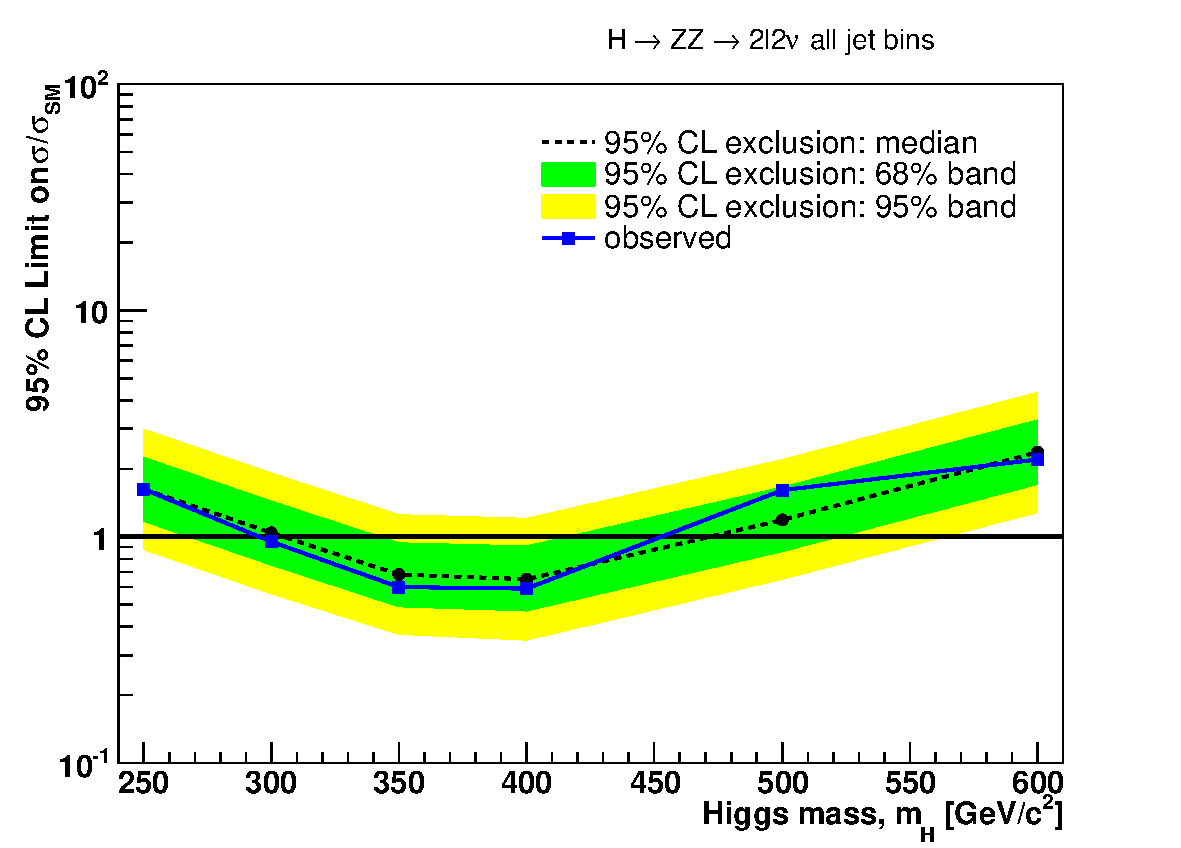
\includegraphics[width=0.5\textwidth]{figures/limits_cut_5fb.pdf}} \\
\end{center}
  \subfigure[$M_T$ Shape Analysis]{
  \centering
  \label{subfig:mtshape}
   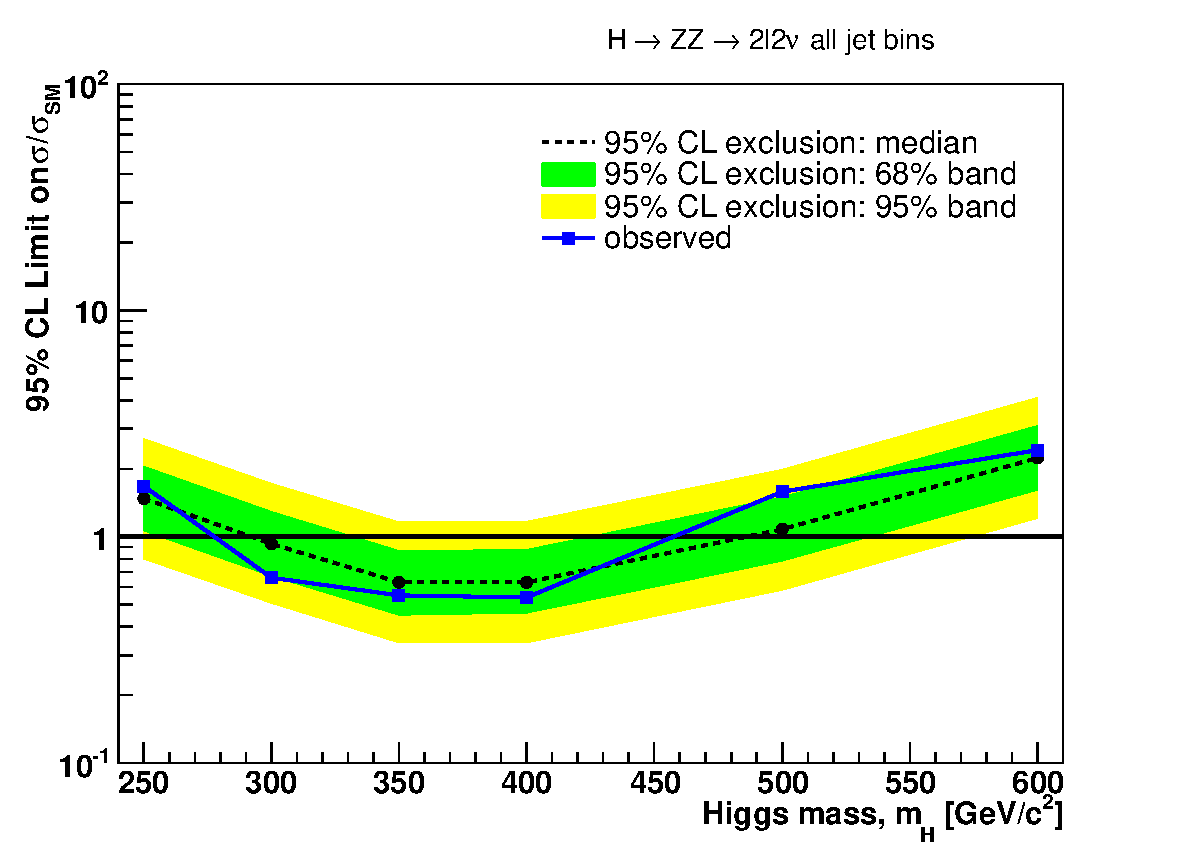
\includegraphics[width=0.5\textwidth]{figures/limits_mtshape_5fb.pdf}}
  \subfigure[Matrix Element Shape Analysis]{
  \centering
  \label{subfig:meshape}
   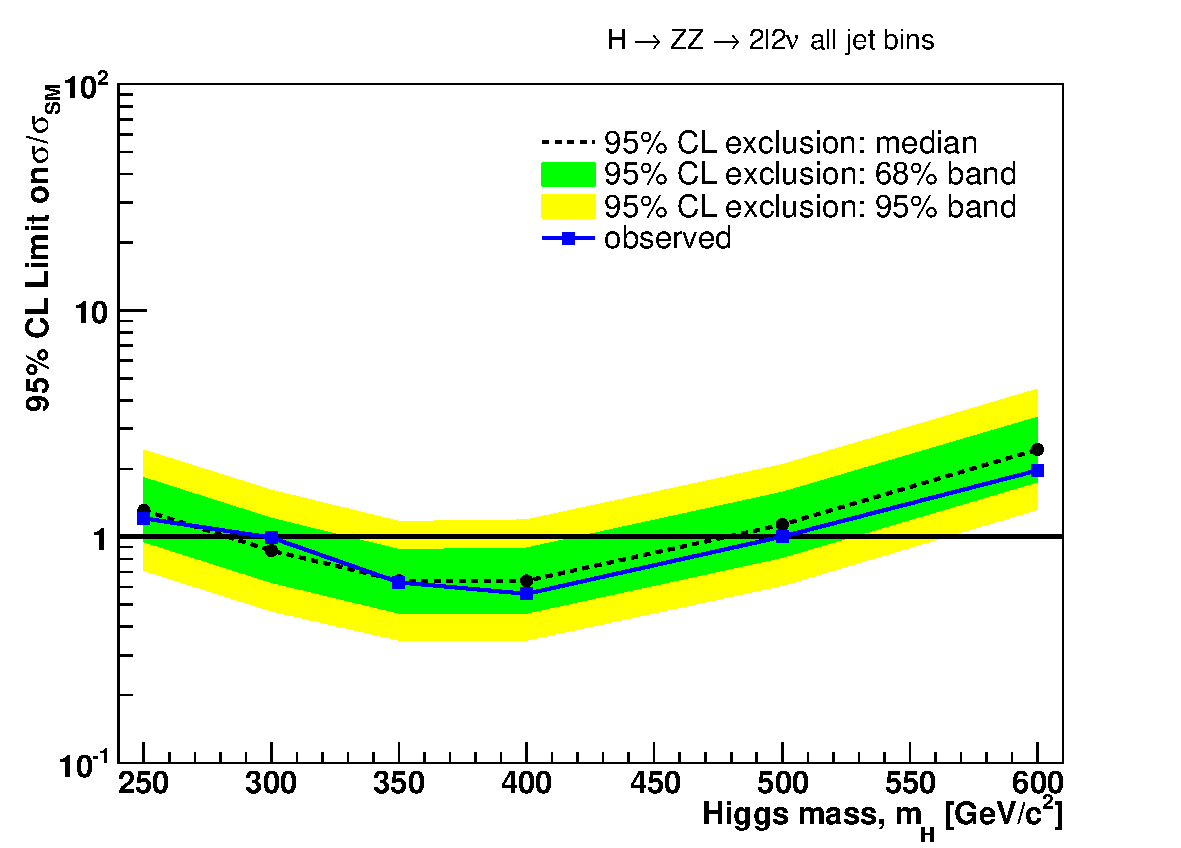
\includegraphics[width=0.5\textwidth]{figures/limits_meshape_5fb.pdf}}
\caption{The expected upper limits at 95\% C.L. for \intlumi\ of data for the 
	cut-based analysis \subref{subfig:cutbased} and 
	shape analysis based on the $M_T$ variable \subref{subfig:mtshape} 
	and matrix element outputs \subref{subfig:meshape}.  
}	
\label{fig:limits_5fb}
\end{figure}
%%%%%%%%%%%%%%%%%%%%%%%%%%%%%


\clearpage
